\section{Results}\label{sec:results}

\subsection{Band-wise expert preferences are reproducible}\label{sec:noisefloor}
Within a band, the top-$k$ expert sets obtained from two disjoint halves of the calibration images agree strongly (Jaccard $0.90$--$0.99$), whereas sets of distant bands agree much less ($0.12$--$0.41$) (Figure~\ref{fig:noisefloor}). Animals and vehicles show the same band structure, so the structure follows the timestep rather than the domain. The load-balance bias term of the router is identically zero in this checkpoint, so selection and weighting are not confounded by load balancing.
This quantifies, with a noise floor, the timestep preference reported qualitatively for a trained DiT-MoE \citep{fei2024ditmoe}. \todo{same measurement on DSMoE-B-E48.}

\begin{figure}[t]\centering
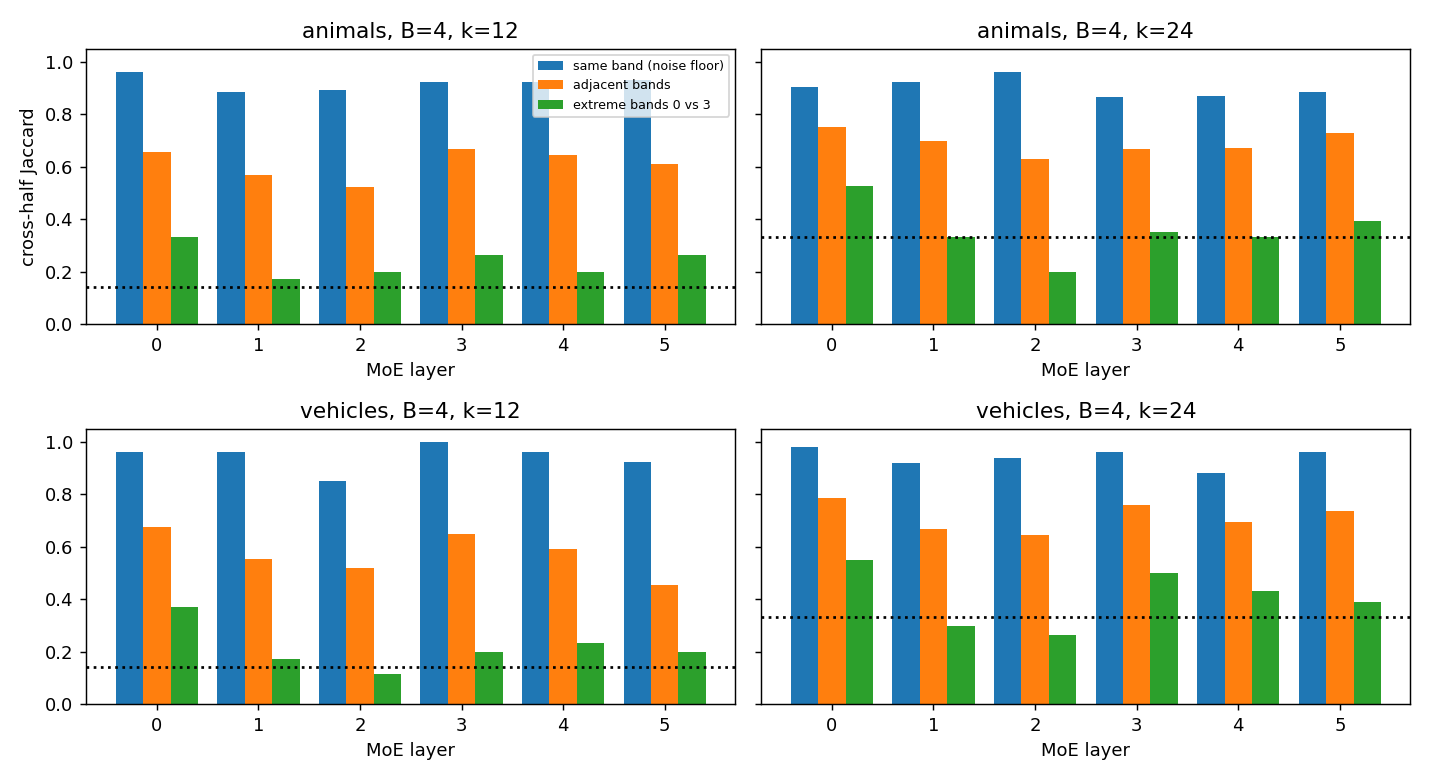
\includegraphics[width=0.9\linewidth]{figures/noisefloor.png}
\caption{Split-half noise floor against between-band overlap of top-$k$ expert sets. \todo{regenerate with final axes/labels and both backbones.}}\label{fig:noisefloor}
\end{figure}

\subsection{Banded versus global selection}\label{sec:bvg}
Table~\ref{tab:main} lists every FID-10k run on the animals domain (baseline $19.141$); $\Delta$ is the increase over the unpruned model, and union is the fraction of routed experts that must be stored statically.

\begin{table}[t]\centering
\caption{Animals domain, FID-10k, single generation seed (seed 0). $B=1$ is global selection. \todo{replace with mean $\pm$ s.d. over seeds for the starred rows and add the baseline-score rows.}}\label{tab:main}
\begin{tabular}{llrrr}
\toprule
$B$ & $k$ & union & FID & $\Delta$ \\
\midrule
1 & 12 & 0.250 & 36.736 & +17.60 \\
1 & 16 & 0.333 & 29.153 & +10.01 \\
1 & 24$^*$ & 0.500 & 22.221 & +3.08 \\
1 & 36$^*$ & 0.750 & 19.654 & +0.51 \\
\midrule
4 & 8  & 0.319 & 46.570 & +27.43 \\
4 & 12 & 0.424 & 31.735 & +12.59 \\
4 & 16 & 0.559 & 25.779 & +6.64 \\
4 & 24$^*$ & 0.747 & 21.277 & +2.14 \\
\midrule
2 & 24 & 0.663 & 21.747 & +2.61 \\
8 & 24 & 0.795 & 21.522 & +2.38 \\
\bottomrule
\end{tabular}
\end{table}

\paragraph{Equal $k$.}
At the same $k$, banded selection ($B=4$) improves on global selection by $0.94$ FID at $k=24$, $3.37$ at $k=16$ and $5.00$ at $k=12$: the advantage grows as the candidate pool shrinks. At $k=24$ the same holds on vehicles ($26.621$ against $27.644$, baseline $24.279$). \todo{error bars; confirm the margins exceed seed noise.}
Under per-band resident memory (Section~\ref{sec:deploy}) equal $k$ is equal resident memory, so this is the relevant comparison there.

\paragraph{Equal static memory.}
Banded selection keeps a different subset per band, so its union is larger than $k/N$: $0.747$ at $k=24$ against $0.500$ for global selection. At matched union, global selection is better in every comparison: global $k=36$ (union $0.750$) reaches FID $19.654$ against $21.277$ for banded $k=24$ (union $0.747$), and global $k=16$ (union $0.333$, $29.153$) beats banded $k=8$ (union $0.319$, $46.570$). Global selection with less memory also beats banded selection with more ($k=16$, union $0.333$: $29.153$, against $B=4$, $k=12$, union $0.424$: $31.735$).
\todo{measured global $k=32$ at union $0.667$ to replace the interpolation against $B=2$, $k=24$.}

\paragraph{Band count.}
At $k=24$, $B\in\{2,4,8\}$ give $21.75$, $21.28$ and $21.52$ against $22.22$ for $B=1$: all banded variants are within about $0.5$ of one another, with no monotone trend in $B$, while paying more union. \todo{significance after seeds.}

\subsection{Does the scoring matter?}\label{sec:scoring}
\todo{random, frequency-only, REAP-style vs full score at $k=24$, $B\in\{1,4\}$; add to Table~\ref{tab:main}.}

\subsection{Calibration with classifier-free guidance}\label{sec:cfg}
Sampling routes both the conditional and the unconditional (null-label) branch, but calibration uses the conditional branch only. The top-$k$ sets obtained from pooled conditional and unconditional statistics overlap with ours at Jaccard $0.90$--$0.99$. \todo{FID of the pooled-calibration selection at $B=4$, $k=24$.}
